\section{第一日第二讲}

{\small\noindent 记录人：Hyun Jong Kim、Han Li\par}

\textbf{算术拓扑}的核心想法是：基本的算术对象（包括环等等）应当表现得像低维流形。下面的表把算术对象列在左列，把类似的拓扑对象列在右列：
\begin{center}
\renewcommand{\arraystretch}{1.35}
\begin{tabular}{c@{\hspace{2.2em}}|@{\hspace{2.2em}}c}
$\mathbb Q$，$\mathbb Z$，$\mathbb Z[i]$，$\mathbb F_p[i]$，$\mathbb F_p$ 上的曲线 $X$ & 3-流形\\
$\mathbb Z[\frac16]$，$\mathbb Z_p$ & 带边 3-流形\\
$\mathbb Q_p$，$\mathbb F_p(\!(t)\!)$，$\mathbb R$，$\mathbb C$，$\overline{\mathbb F}_p$ 上的曲线 $X$ & 2-流形\\
$\overline{\mathbb F}_p(\!(t)\!)$ & 1-流形\\
理想 & 链环\\
素理想 & 纽结\\
$\mathcal O_{\mathfrak p}$ & $\mathfrak p$ 的管状邻域
\end{tabular}
\end{center}

这些类比的动机之一，是流形的 $\pi_1$ 与概形的平展基本群之间的类比。

\textbf{历史}\enspace 大约在 1880 年，Dedekind 不满意 Riemann 对 Riemann 曲面的（不够精确的）定义。于是他同 Weber 合写了一篇文章，其中给出了 Riemann 曲面的定义。他看出：Riemann 曲面的分歧覆盖 $\Sigma\to\Sigma'$ 类似于数域的扩张 $L/K$。

1949 年，Weil 猜想应当存在一种纯代数的方式来研究代数簇的拓扑。也就是说，对复代数簇 $X=\Spec R$，应当有一种只从 $R$ 本身算出 $H^*(X(\mathbb C))$ 的办法。特别地，$R$ 的 $\mathbb C$-自同构——包括那些极其疯狂的、来自 $\mathbb C$ 的算术而非 $X$ 的几何的自同构——应当诱导 $H^*(X)$ 的 $\mathbb C$-自同构。这一点由 Grothendieck 学派用平展拓扑 $H^*_{\text{ét}}(R)$ 实现。

1960 年代，Poitou 与 Tate 对 $R=\mathbb Z[\frac1p]$ 等情形算出了 $H^*_{\text{ét}}(R)$。Mumford 与 Mazur 提出：$\Spec\mathbb Z$ 就像一个 3-流形。

\medskip
\noindent\textbf{例}\enspace 设 $K$ 是数域，$S$ 是包含所有 Archimedean 位的有限位点集，$\mathcal O$ 是 $K$ 的整数环；或者另一个情形：$K=X(\mathbb F_q)$，$X$ 是光滑射影曲线，$\mathcal O$ 是「在 $S$ 之外正则」的函数环。例如 $K=\mathbb Q$、$S=\{\infty,2\}$、$\mathcal O=\mathbb Z[\frac12]$。设 $M$ 是一个系数系统。

则存在长正合列：
\begin{equation}
\begin{split}
\cdots&\to H^{3-i}_{\text{ét}}(\Spec\mathcal O,M^*)^*\to H^i_{\text{ét}}(\Spec\mathcal O;M)\to\bigoplus_{\nu\in S}H^i_{\text{ét}}(\Spec K_\nu;M)\\
&\to H^{3-(i+1)}_{\text{ét}}(\Spec\mathcal O,M^*)^*\to\cdots
\end{split}
\label{eq:arith}
\end{equation}
（若 $M$ 有限，则 $M^*=\Hom(M,S^1)$。一般地，$*$ 所涉及的扭转对应于流形的不可定向性。）

\medskip
这与上同调的长正合列类似，其中 $X$ 是边界为 $Y$ 的 3-流形：
\begin{equation}
\cdots\to H^i(X,Y;M)\to H^i(X;M)\to H^i(Y;M)\to\cdots .
\label{eq:top}
\end{equation}

在 Poincaré 对偶 $H_i(X,Y;M)\cong H^{3-i}(X;M^*)^*$ 之下，上面的长正合列 \eqref{eq:top} 变成
\[
\cdots\to H^{3-i}(X;M^*)^*\to H^i(X;M)\to H^i(Y;M)\to\cdots,
\]
它与 \eqref{eq:arith} 类似。注意右侧没有 $Y$：$X$「知道」$\partial X$ 是什么。这就是 Poincaré--Lefschetz 对偶。

于是这个类比提示：$\Spec\mathcal O$ 像一个（不可定向的）3-流形，其边界是 $\bigsqcup_{\nu\in S}\Spec K_\nu$，见图 \ref{fig:specO}。

\begin{figure}[htbp]
  \centering
  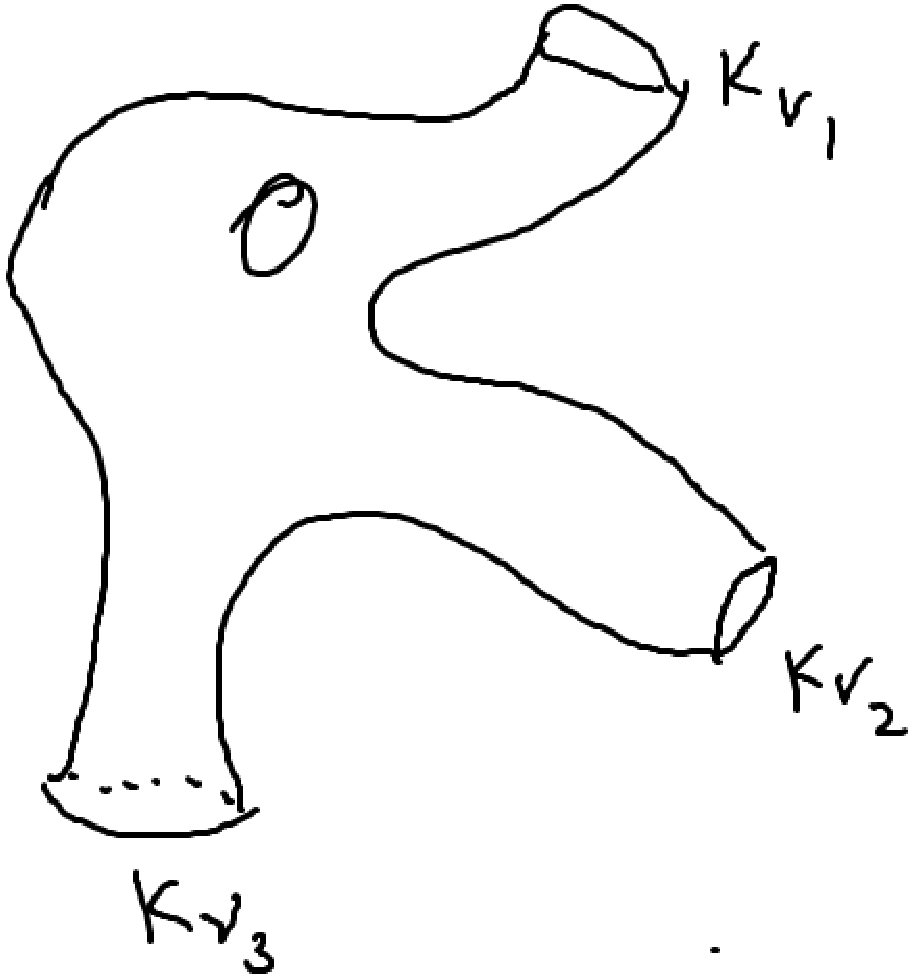
\includegraphics[width=0.30\textwidth]{f21-specO.png}
  \caption{$\Spec\mathcal O$ 类似于一个 3-流形，其边界是 $\bigsqcup_{\nu\in S}\Spec K_\nu$}
  \label{fig:specO}
\end{figure}

当然，作为一个拓扑空间，$\Spec\mathcal O$ 并不是 3 维的。更一般地，我们要强调：本讲义里记录下来的这些几何类比只是类比，我们并不是在把它们当作关于概形或空间的精确事实来陈述。

在 $\mathcal O=\mathbb Z[\frac12]$ 的例子中，$\Spec\mathbb Z[\frac12]$ 有两个边界分支，即 $\Spec\mathbb R$ 与 $\Spec\mathbb Q_2$，见图 \ref{fig:specZ12}。此外，素理想像纽结/循环——图 \ref{fig:knot} 把 $\mathbb Z[\frac12]$ 的素理想 $(3)$ 画成一个纽结/循环。

\begin{figure}[htbp]
  \centering
  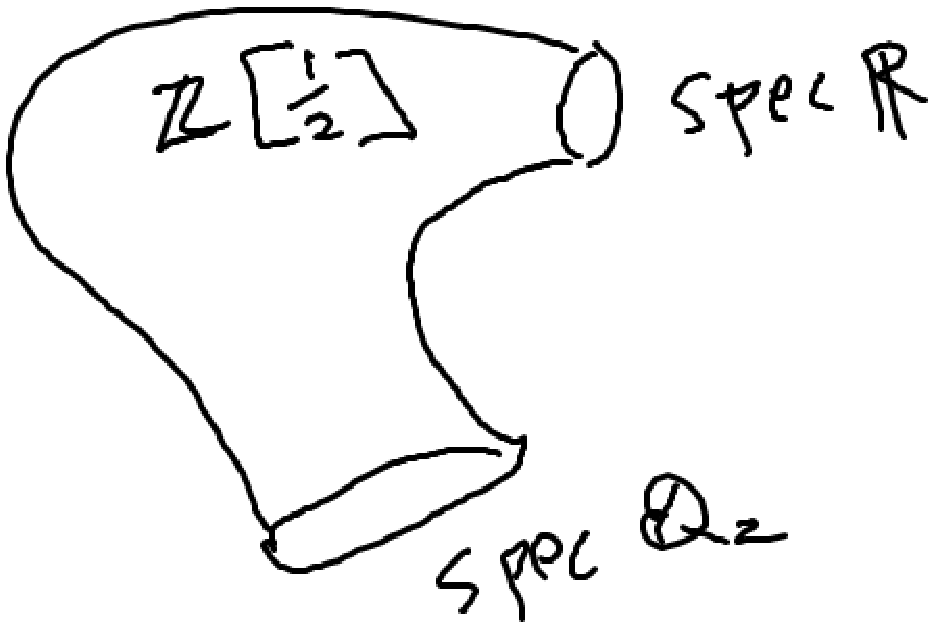
\includegraphics[width=0.30\textwidth]{f22-specZ12.png}
  \caption{$\Spec\mathbb Z[\frac12]$ 类似于一个 3-流形，其边界是 $\Spec\mathbb Q_2\sqcup\Spec\mathbb R$}
  \label{fig:specZ12}
\end{figure}

从 $\Spec\mathbb Z[\frac12]$ 出发，把与素理想 $3\mathbb Z$ 对应的纽结周围的管状邻域挖掉，就得到 $\Spec\mathbb Z[\frac16]$；这里所说的实心管是 $\Spec\mathbb Z_3$，其边界是 $\Spec\mathbb Q_3$，见图 \ref{fig:tube}。换言之，沿 $\Spec\mathbb Q_3$ 把 $\Spec\mathbb Z_3$ 粘到 $\Spec\mathbb Z[\frac16]$ 上，就得到 $\Spec\mathbb Z[\frac12]$。

\begin{figure}[htbp]
  \centering
  \begin{minipage}[t]{0.32\textwidth}
    \centering
    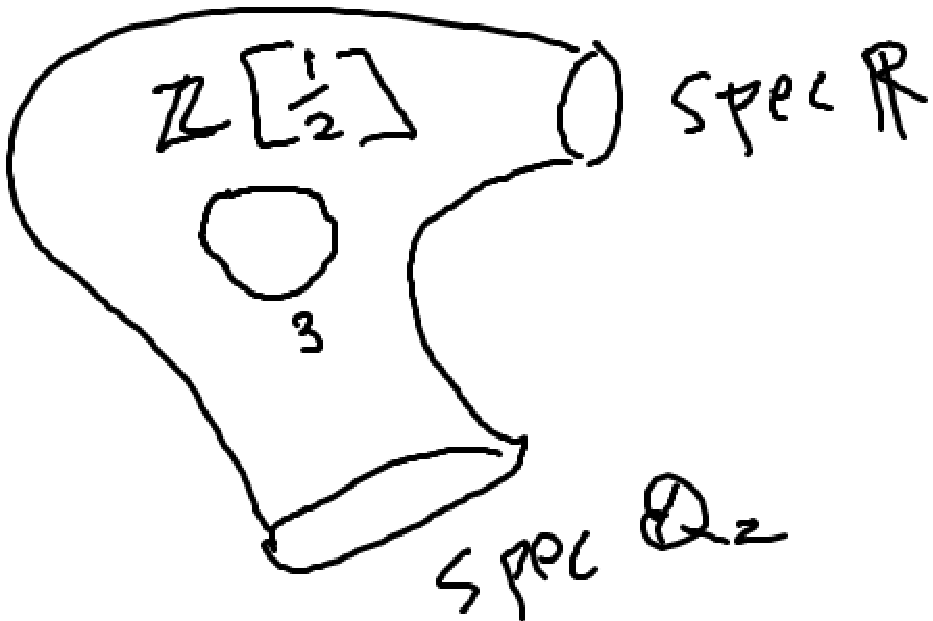
\includegraphics[width=\textwidth]{f23-knot.png}
    \caption{$\Spec\mathbb Z[\frac12]$ 的素理想 $(3)$ 类似于 3-流形中的一个纽结/循环}
    \label{fig:knot}
  \end{minipage}\hfill
  \begin{minipage}[t]{0.32\textwidth}
    \centering
    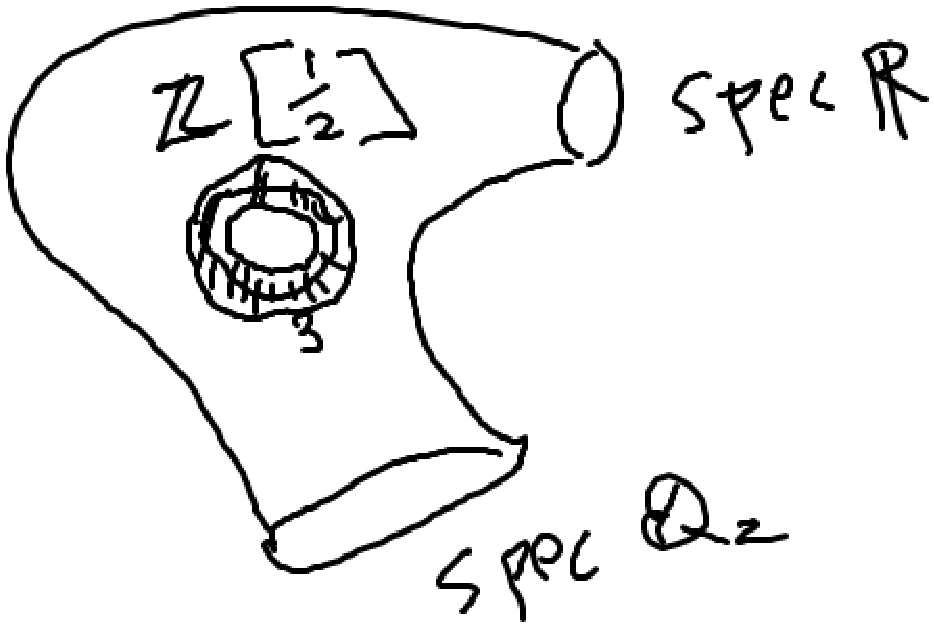
\includegraphics[width=\textwidth]{f24-tube.png}
    \caption{在对应于 $\mathbb Z[\frac12]$ 的素理想 $(3)$ 的纽结周围画出实心管；把这根实心管挖掉就得到 $\mathbb Z[\frac16]$}
    \label{fig:tube}
  \end{minipage}
\end{figure}

\textbf{Langlands 作为 4 维 TQFT}\enspace 字典里没有 4-流形，所以我们从「把向量空间配给类似于 3-流形的算术对象」开始：
\begin{center}
\begin{tabular}{rcl}
「3-流形」 & $\mapsto$ & 向量空间\\
「2-流形」 & $\mapsto$ & 范畴\\
「1-流形」 & $\mapsto$ & 2-范畴
\end{tabular}
\end{center}

例如对 $G=\operatorname{SL}_n$（问题：若 $G$ 不是 $\operatorname{SL}_n$，下面的一切会变吗？），这个「TQFT」$A_G$ 的作用如下：
\[
\begin{array}{r@{\quad}l}
\text{3d} &
\begin{cases}
\mathbb Z\mapsto G(\mathbb Z)\backslash G(\mathbb R)\ \text{上的函数，即自守形式}\\[1pt]
\mathbb Z[\tfrac1p]\mapsto G(\mathbb Z[\tfrac1p])\backslash\bigl(G(\mathbb R)\times G(\mathbb Q_p)\bigr)\ \text{上的函数}\\[1pt]
\mathbb F_p\ \text{上的曲线}\ X\mapsto \Bun_G X\ \text{上的函数}
\end{cases}\\[22pt]
\text{2d} &
\begin{cases}
\mathbb R\ \text{或}\ \mathbb Q_p\mapsto \Rep G(\mathbb R)\ \text{或}\ \Rep G(\mathbb Q_p)\quad\text{（局部 Langlands）}\\[1pt]
\overline{\mathbb F}_p\ \text{上的曲线}\ X\mapsto \Shv(\Bun_G X)\quad\text{（整体几何 Langlands）}
\end{cases}
\end{array}
\]

在配边一侧，$\partial\mathbb Z[\frac1p]=\mathbb R\sqcup\mathbb Q_p$；在代数一侧，
$\{G(\mathbb Z[\frac1p])\backslash(G(\mathbb R)\times G(\mathbb Q_p))\ \text{上的函数}\}\in\Rep\bigl(G(\mathbb R)\times G(\mathbb Q_p)\bigr)$（正则表示）。这与 4 维 TQFT 里带边流形的工作方式一致：带边的 3-流形应当被送到一个范畴连同其中一个对象。

至于复合，由于 $\Spec\mathbb Z[\frac1p]\cup_{\Spec\mathbb Q_p}\Spec\mathbb Z_p=\Spec\mathbb Z$，我们期望
\[
A_G(\mathbb Z)=\Hom_{\Rep G(\mathbb Q_p)}\bigl(A_G(\mathbb Z_p),A_G(\mathbb Z[\tfrac1p])\bigr),
\]
（或者反过来，但那样行不通）。这就迫使 $A_G(\mathbb Z_p)=\operatorname{ind}_{G(\mathbb Z_p)}^{G(\mathbb Q_p)}\mathbf 1$（按定义，$\operatorname{ind}_H^G\rho=\{\phi:G\to V:\phi(gh^{-1})=\rho(h)\phi(g);\ \phi\ \text{模}\ H\ \text{有紧支集}\}$）。

这也说明 $\operatorname{End}_{\Rep G(\mathbb Q_p)}A_G(\mathbb Z_p)$ 作用在 $A_G(\mathbb Z)$ 上（通过复合）。事实上 $\operatorname{End}_{\Rep G(\mathbb Q_p)}A_G(\mathbb Z_p)$ 就是 $G(\mathbb Q_p)$ 的（无分歧）Hecke 代数。因此 $A_G$ 里已经内建了一大堆算子。

\textbf{互反性}\enspace Langlands 纲领的中心猜想之一是「互反」，即一个双射
\[
\{\text{Hecke 算子的特征函数}\}\longleftrightarrow\{\text{同态}\ \pi_1(\text{算术对象})\to\check G\}.
\]
记作 $A_G\xrightarrow{\sim}B_{\check G}$。

$A_G\xrightarrow{\sim}B_{\check G}$ 是上述算术 TQFT $A_G$ 与另一个算术 TQFT $B_{\check G}$ 之间的等价。断言这两个算术 TQFT 等价，就把 Langlands 纲领的各个层次编码在一起——代入数域、局部域等等，就得到相应类型的双射。这种表述的好处，不在于能得到新陈述（因为特化到每个算术对象时，得到的都是已知陈述），而在于它给出一种统一的方式来谈论贯穿 Langlands 纲领的现象，而不必把各种情形分开处理。人们可以在 Langlands 纲领的不同部分还原出许多不同的方面与陈述。相对 Langlands 对偶是类似的现象——它存在于 Langlands 纲领的每一层——因此上述等价是一个有用的方式，用来在头脑中组织并追踪各层之间的关系。

\medskip
\noindent\textbf{练习 1}\enspace
\begin{enumerate}[label=(\alph*),leftmargin=2.0em,itemsep=0.35em,topsep=0.2em]
\item 我们需要验证
\[
\sum_i q^{-\frac i2}\operatorname{tr}\bigl(g\,\big|\,\mathbb C[Y]_i\bigr)=\frac{1}{(1-q^{-\frac12}x)(1-q^{-\frac12}x^{-1})}.
\]
右端是两个几何级数之积。$q^{-\frac i2}$ 的系数是 $x^{-i}+x^{-i+2}+\cdots+x^i$，它应当等于 $\operatorname{tr}\bigl(x\,\big|\,\mathbb C[Y]_i\bigr)$。

$\mathbb C[Y]=\mathbb C[T^*\mathbb A^1]=\mathbb C[q,p]$。对 $f\in\mathbb C[q,p]$，有 $x\cdot f(q,p)=f\bigl((q,p)\cdot x\bigr)=f(xq,x^{-1}p)$；特别地 $x\cdot q=xq$、$x\cdot p=x^{-1}p$。

$\mathbb C[Y]_i$ 的一组基是 $\{q^ip^0,\dots,q^0p^i\}$；在 $x$ 的作用下它变成 $\{x^iq^ip^0,\dots,x^{-i}q^0p^i\}$。因此 $\bigl.x\bigr|_{\mathbb C[Y]_i}$ 是对角矩阵，迹为 $x^i+x^{i-2}+\cdots+x^{-i}$。
\item 等价地，$x\in\mathbb C^*$ 现在对角地作用在 $Y^2$ 上。
\item $\operatorname{Ad}_g\begin{pmatrix}a&b\\c&d\end{pmatrix}=\begin{pmatrix}a&x^2b\\x^{-2}c&d\end{pmatrix}$。因此，等价地，$x^2\in\mathbb C^*$ 作用在 $Y\times Y$ 上，在第一个 $Y$ 上平凡作用，在第二个 $Y$ 上按 (a) 的方式作用。
\end{enumerate}
